% For LaTeX-Box: root = DMC2015_introduction.tex 
%%%%%%%%%%%%%%%%%%%%%%%%%%%%%%%%%%%%%%%%%%%%%%%%%%%%%%%%%%%%%%%%%%%%%%%%%%%%%%%%
%  File Name: DMC2015_introduction.tex
%  Purpose:
%
%  Creation Date: 31-03-2015
%  Last Modified: Tue Mar 31 18:08:29 2015
%  Created By:
%%%%%%%%%%%%%%%%%%%%%%%%%%%%%%%%%%%%%%%%%%%%%%%%%%%%%%%%%%%%%%%%%%%%%%%%%%%%%%%%
%  To start a homework: :r ~/TeX/hwtemplate.tex
\documentclass[xcolor=dvipsnames,gray,mathserif]{beamer}
\usetheme{Boadilla}
\usepackage{graphicx}
\usepackage{graphics}
\usepackage{epsfig}
\usepackage{amsmath,amssymb} % \fleqn if taken out math environments will get centered
\usepackage{tikz}
\usetikzlibrary{backgrounds}
%\documentclass[11pt,red]{beamer}

%\usepackage{inc/inc}
\usepackage{amsmath,amssymb,amsfonts,amscd}
\usepackage{graphicx,bm,booktabs,subfigure}

\usepackage{url}
\usepackage{textcomp}
\usepackage[vcentermath]{youngtab}

\usepackage{multirow}
\usepackage{epsfig}
\usepackage{latexsym}
\usepackage{amssymb}
%\usepackage{amstex}
\usepackage{amstext}
\usepackage{amsgen}
\usepackage{amsxtra}
\usepackage{amsgen}
\usepackage{amsthm}
\usepackage{color}

\usepackage{chemarr}
\usepackage[mathscr]{eucal}
\usepackage{xspace}
\usepackage{setspace}
\usepackage{booktabs}


\newcommand{\M}{\operatorname{M}}
\newcommand{\mr}{\operatorname{mr}}

% notation related to skew min rank
\newcommand{\s}{\mathcal{S}}
\newcommand{\sS}{\mathcal{S}^-}
\newcommand{\smr}{\operatorname{mr}^-}
\newcommand{\sMR}{\operatorname{MR}^-}
\newcommand{\sM}{\operatorname{M}^-}
\newcommand{\sZ}{\operatorname{Z}^-}
\newcommand{\srv}{\operatorname{r}_v^-}
\newcommand{\G}{\mathcal{G}}
\newcommand{\R}{\mathbb{R}}

% notation related to theorems etc.
\newtheorem{thm}{Theorem}
\newtheorem{defn}[thm]{Definition}
\newtheorem{prop}[thm]{Proposition}
\newtheorem{cor}[thm]{Corollary}
\newtheorem{lem}[thm]{Lemma}
\newtheorem{remark}[thm]{Remark}
\newtheorem{conj}[thm]{Conjecture}
\newtheorem{ex}[thm]{Example}
\newtheorem{quest}[thm]{Question}
\newtheorem{obs}[thm]{Observation}
\newtheorem{prog}[thm]{Program Call}

% matrix and order
\def\mtx#1{\begin{bmatrix} #1 \end{bmatrix}}
\def\ord#1{| #1 |}

% notation related to vectors and rank
\newcommand{\bb}{{\bf b}}
\newcommand{\bv}{{\bf v}}
\newcommand{\x}{{\bf x}}
\newcommand{\y}{{\bf y}}
\newcommand{\rank}{\operatorname{rank}}
\newcommand{\match}{\operatorname{match}}
\newcommand{\dotcup}{\dot{\cup}}

\definecolor{myBlue}{rgb}{0.1,0.1,0.45098039}
\def\Head#1{\noindent{\color{myBlue} #1}}

\date[Apr 23, 2013]{Apr 23, 2013}

\definecolor{myBlue}{rgb}{0.1,0.1,0.45098039}
\def\Head#1{\noindent{\color{myBlue} #1}}

%%%% FANCY QUOTES %%%
\makeatletter
\tikzset{%
  fancy quotes/.style={
    text width=\fq@width pt,
    align=justify,
    inner sep=1em,
    anchor=north west,
    minimum width=\textwidth,
  },
  fancy quotes width/.initial={.8\textwidth},
  fancy quotes marks/.style={
    scale=8,
    text=white,
    inner sep=0pt,
  },
  fancy quotes opening/.style={
    fancy quotes marks,
  },
  fancy quotes closing/.style={
    fancy quotes marks,
  },
  fancy quotes background/.style={
    show background rectangle,
    inner frame xsep=0pt,
    background rectangle/.style={
      fill=gray!25,
      rounded corners,
    },
  }
}

\newenvironment{fancyquotes}[1][]{%
\noindent
\tikzpicture[fancy quotes background]
\node[fancy quotes opening,anchor=north west] (fq@ul) at (0,0) {``};
\tikz@scan@one@point\pgfutil@firstofone(fq@ul.east)
\pgfmathsetmacro{\fq@width}{\textwidth - 2*\pgf@x}
\node[fancy quotes,#1] (fq@txt) at (fq@ul.north west) \bgroup}
{\egroup;
\node[overlay,fancy quotes closing,anchor=east] at (fq@txt.south east) {''};
\endtikzpicture}
\makeatother
%%% End of fancy quotes


\newcommand{\blue}[1]{{\color{blue} #1}}
\newcommand{\red}[1]{{\color{red} #1}}
\newcommand{\normal}{\mathcal{N}}
\setbeamercovered{transparent}

\title[The 2015 Data Mining Cup]{DMC 2015}
\subtitle{So You Want To Be A Data Miner?}
\author[ISU Team]{ISU Team}

\date{April and May, 2015}
\institute[ISU Team]{Presentation by Ian Mouzon}

\begin{document}
\begin{frame}
\titlepage
\end{frame}

\begin{frame}
\frametitle{The Data Mining Cup}
\framesubtitle{What is it?}
The Data Mining Cup is a yearly competition hosted by prudsys (all lower case) a German analytics company
focused on marketplace behavior. 

\vspace{.5cm}

\begin{fancyquotes}
The DATA MINING CUP (DMC for short) has been inspiring students around the world to pursue intelligent data analysis since the year 2000.
In 2014 over one thousand students from about 100 universities in 28 countries took part in the competition.
The best teams will be invited to Berlin for the awards ceremony at the prudsys personalization summit.
\end{fancyquotes}
\end{frame}

\begin{frame}
\frametitle{What is ISU's history in the DMC}
\framesubtitle{Fifth Place in 2013 DMC}
In 2013 we had six team members (all from the STAT department and most associated in some way with Dr. Vardeman and STAT 602).
\centerline{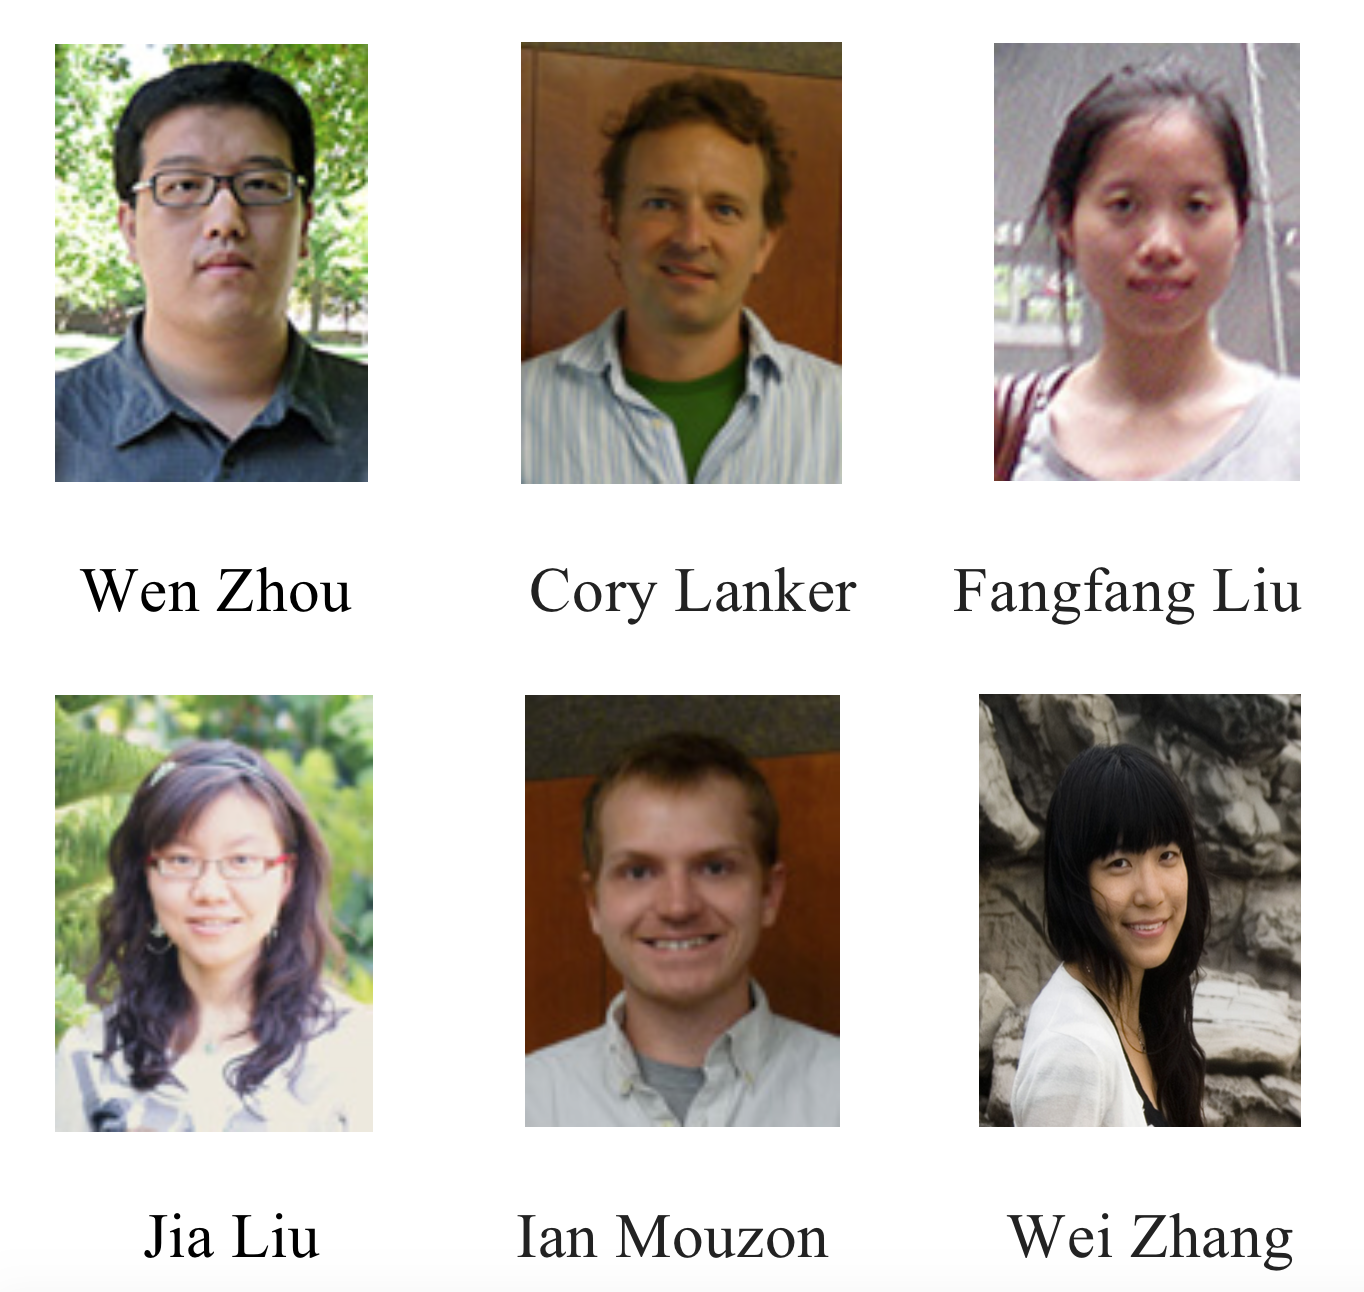
\includegraphics[height=.3\linewidth]{./figs/team2013}}
Our team came in fifth place and some of our members were able to travel to Berlin for the awards ceremony.
\end{frame}

\begin{frame}
\frametitle{What is ISU's history in the DMC}
\framesubtitle{Fifth Place Goes to Germany}
\centerline{
   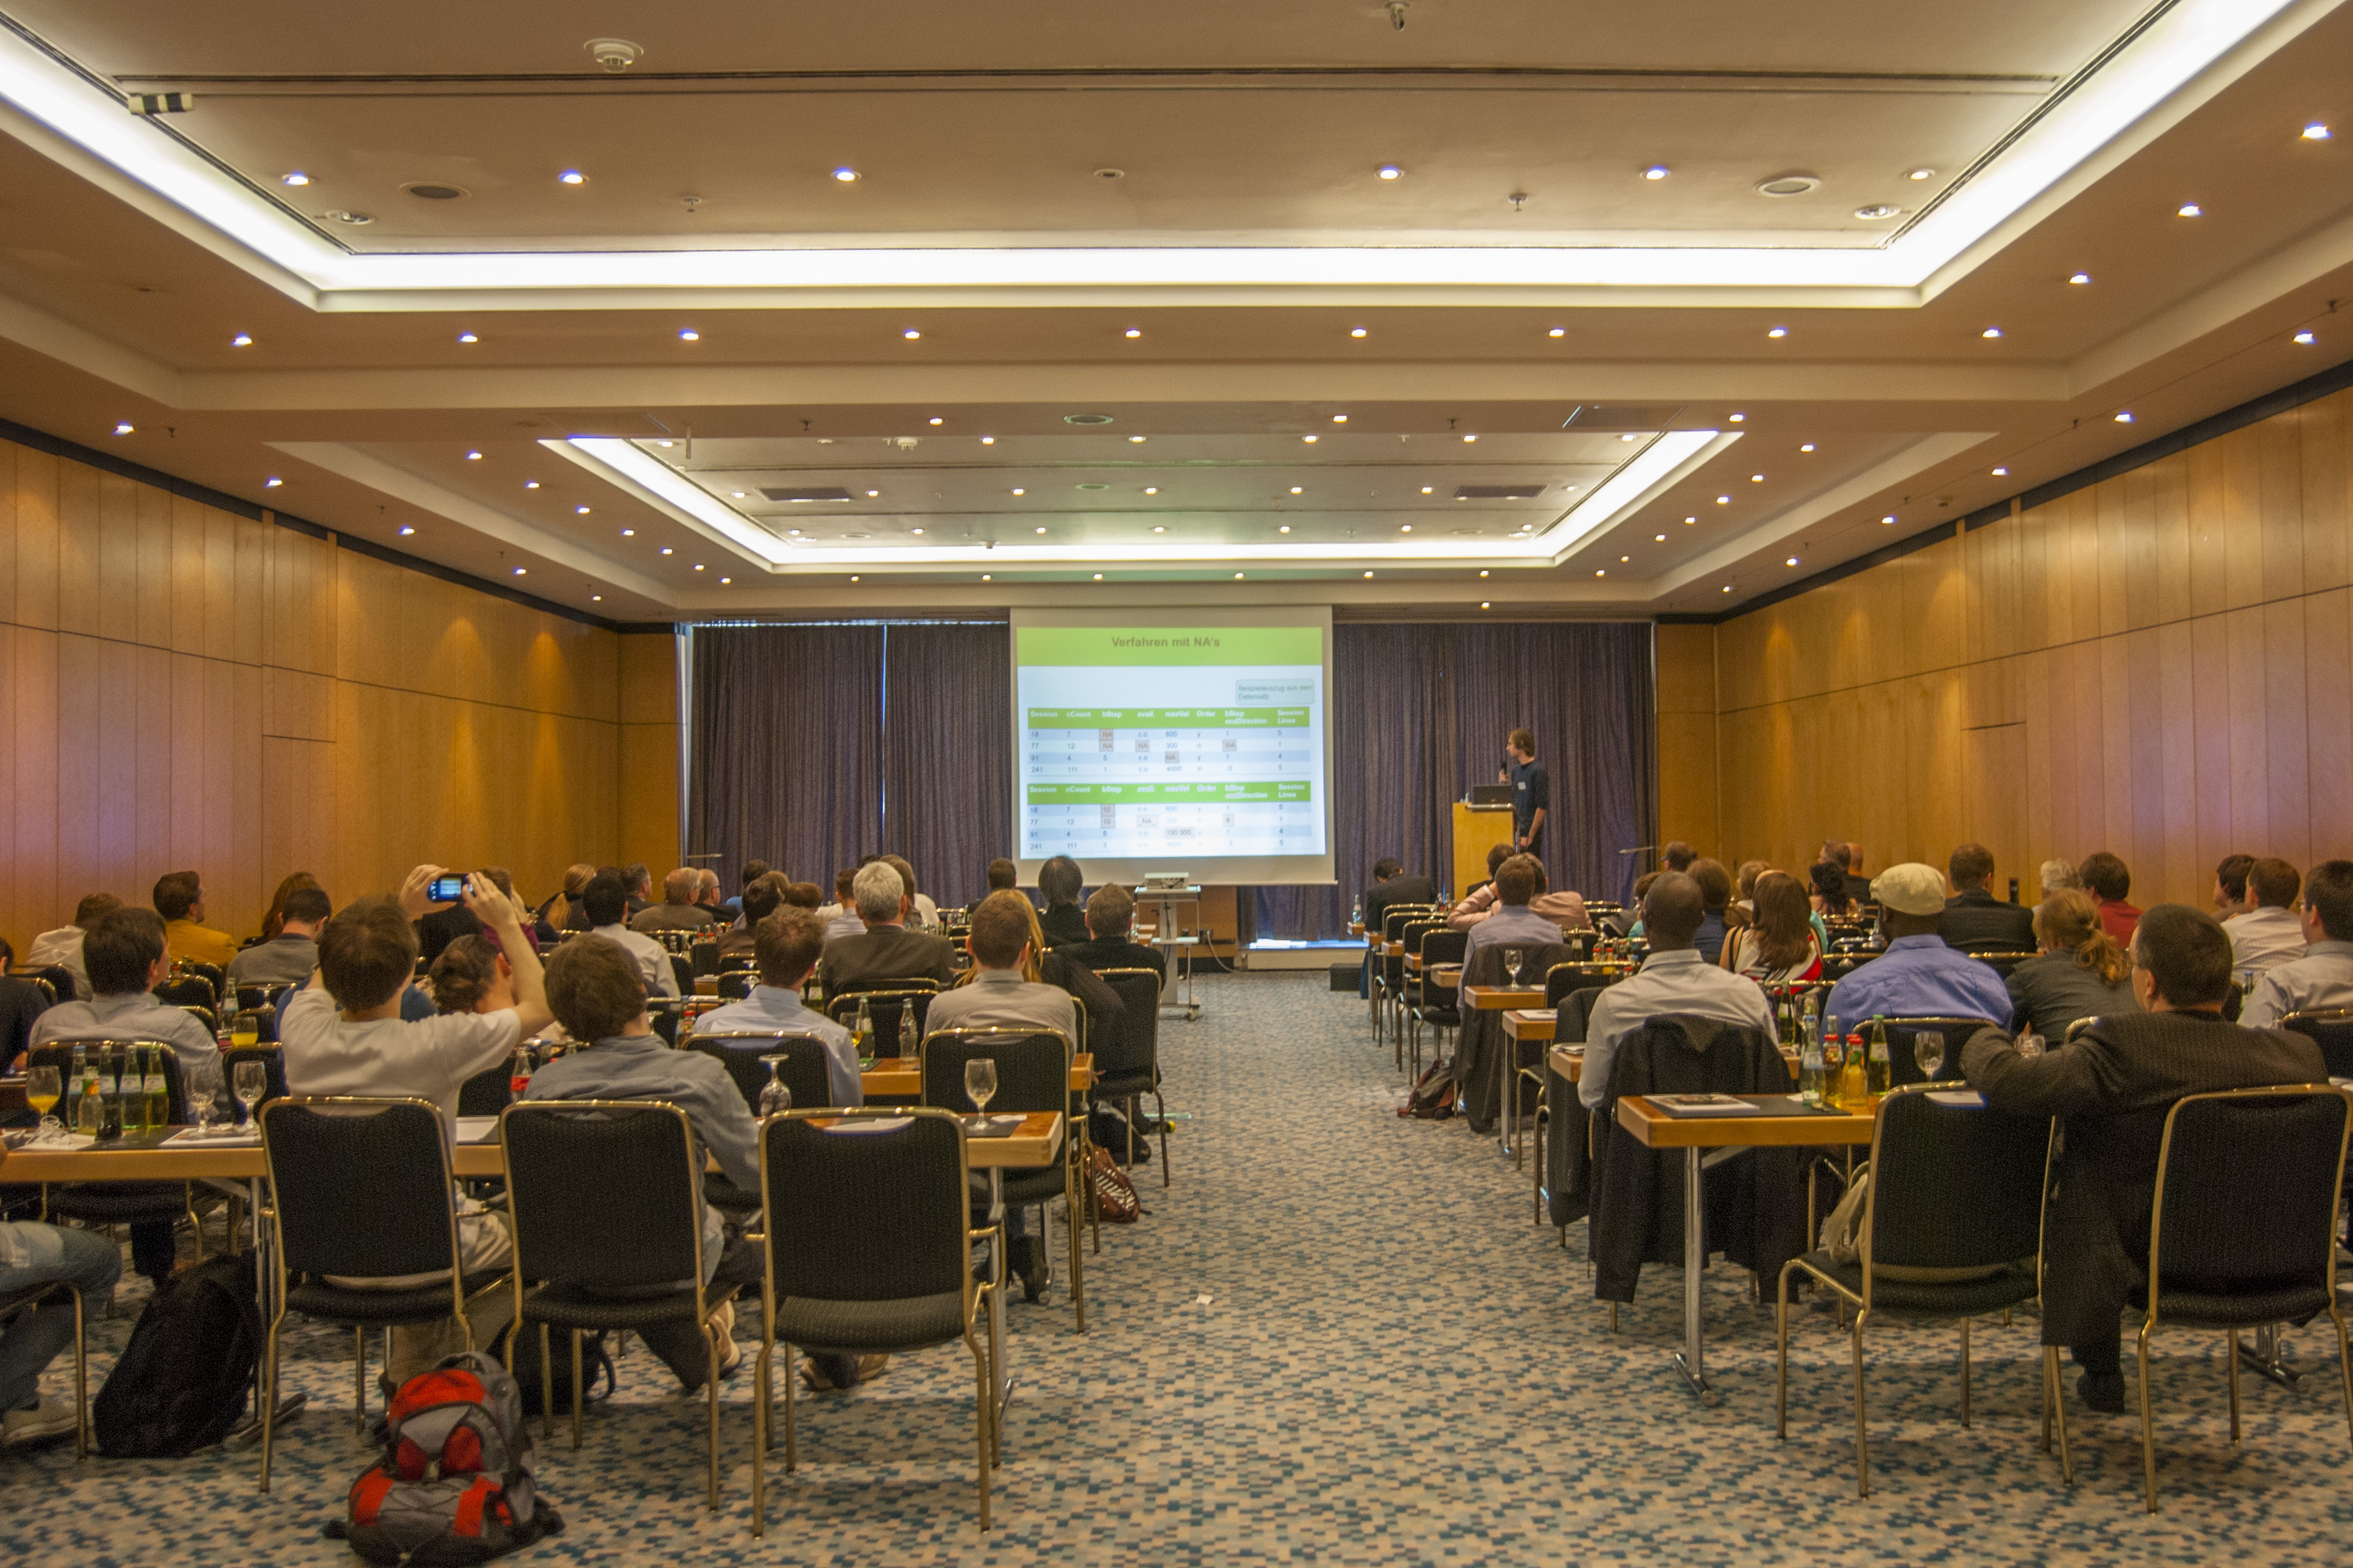
\includegraphics[width=.3\linewidth]{./figs/ceremony_2013} 
   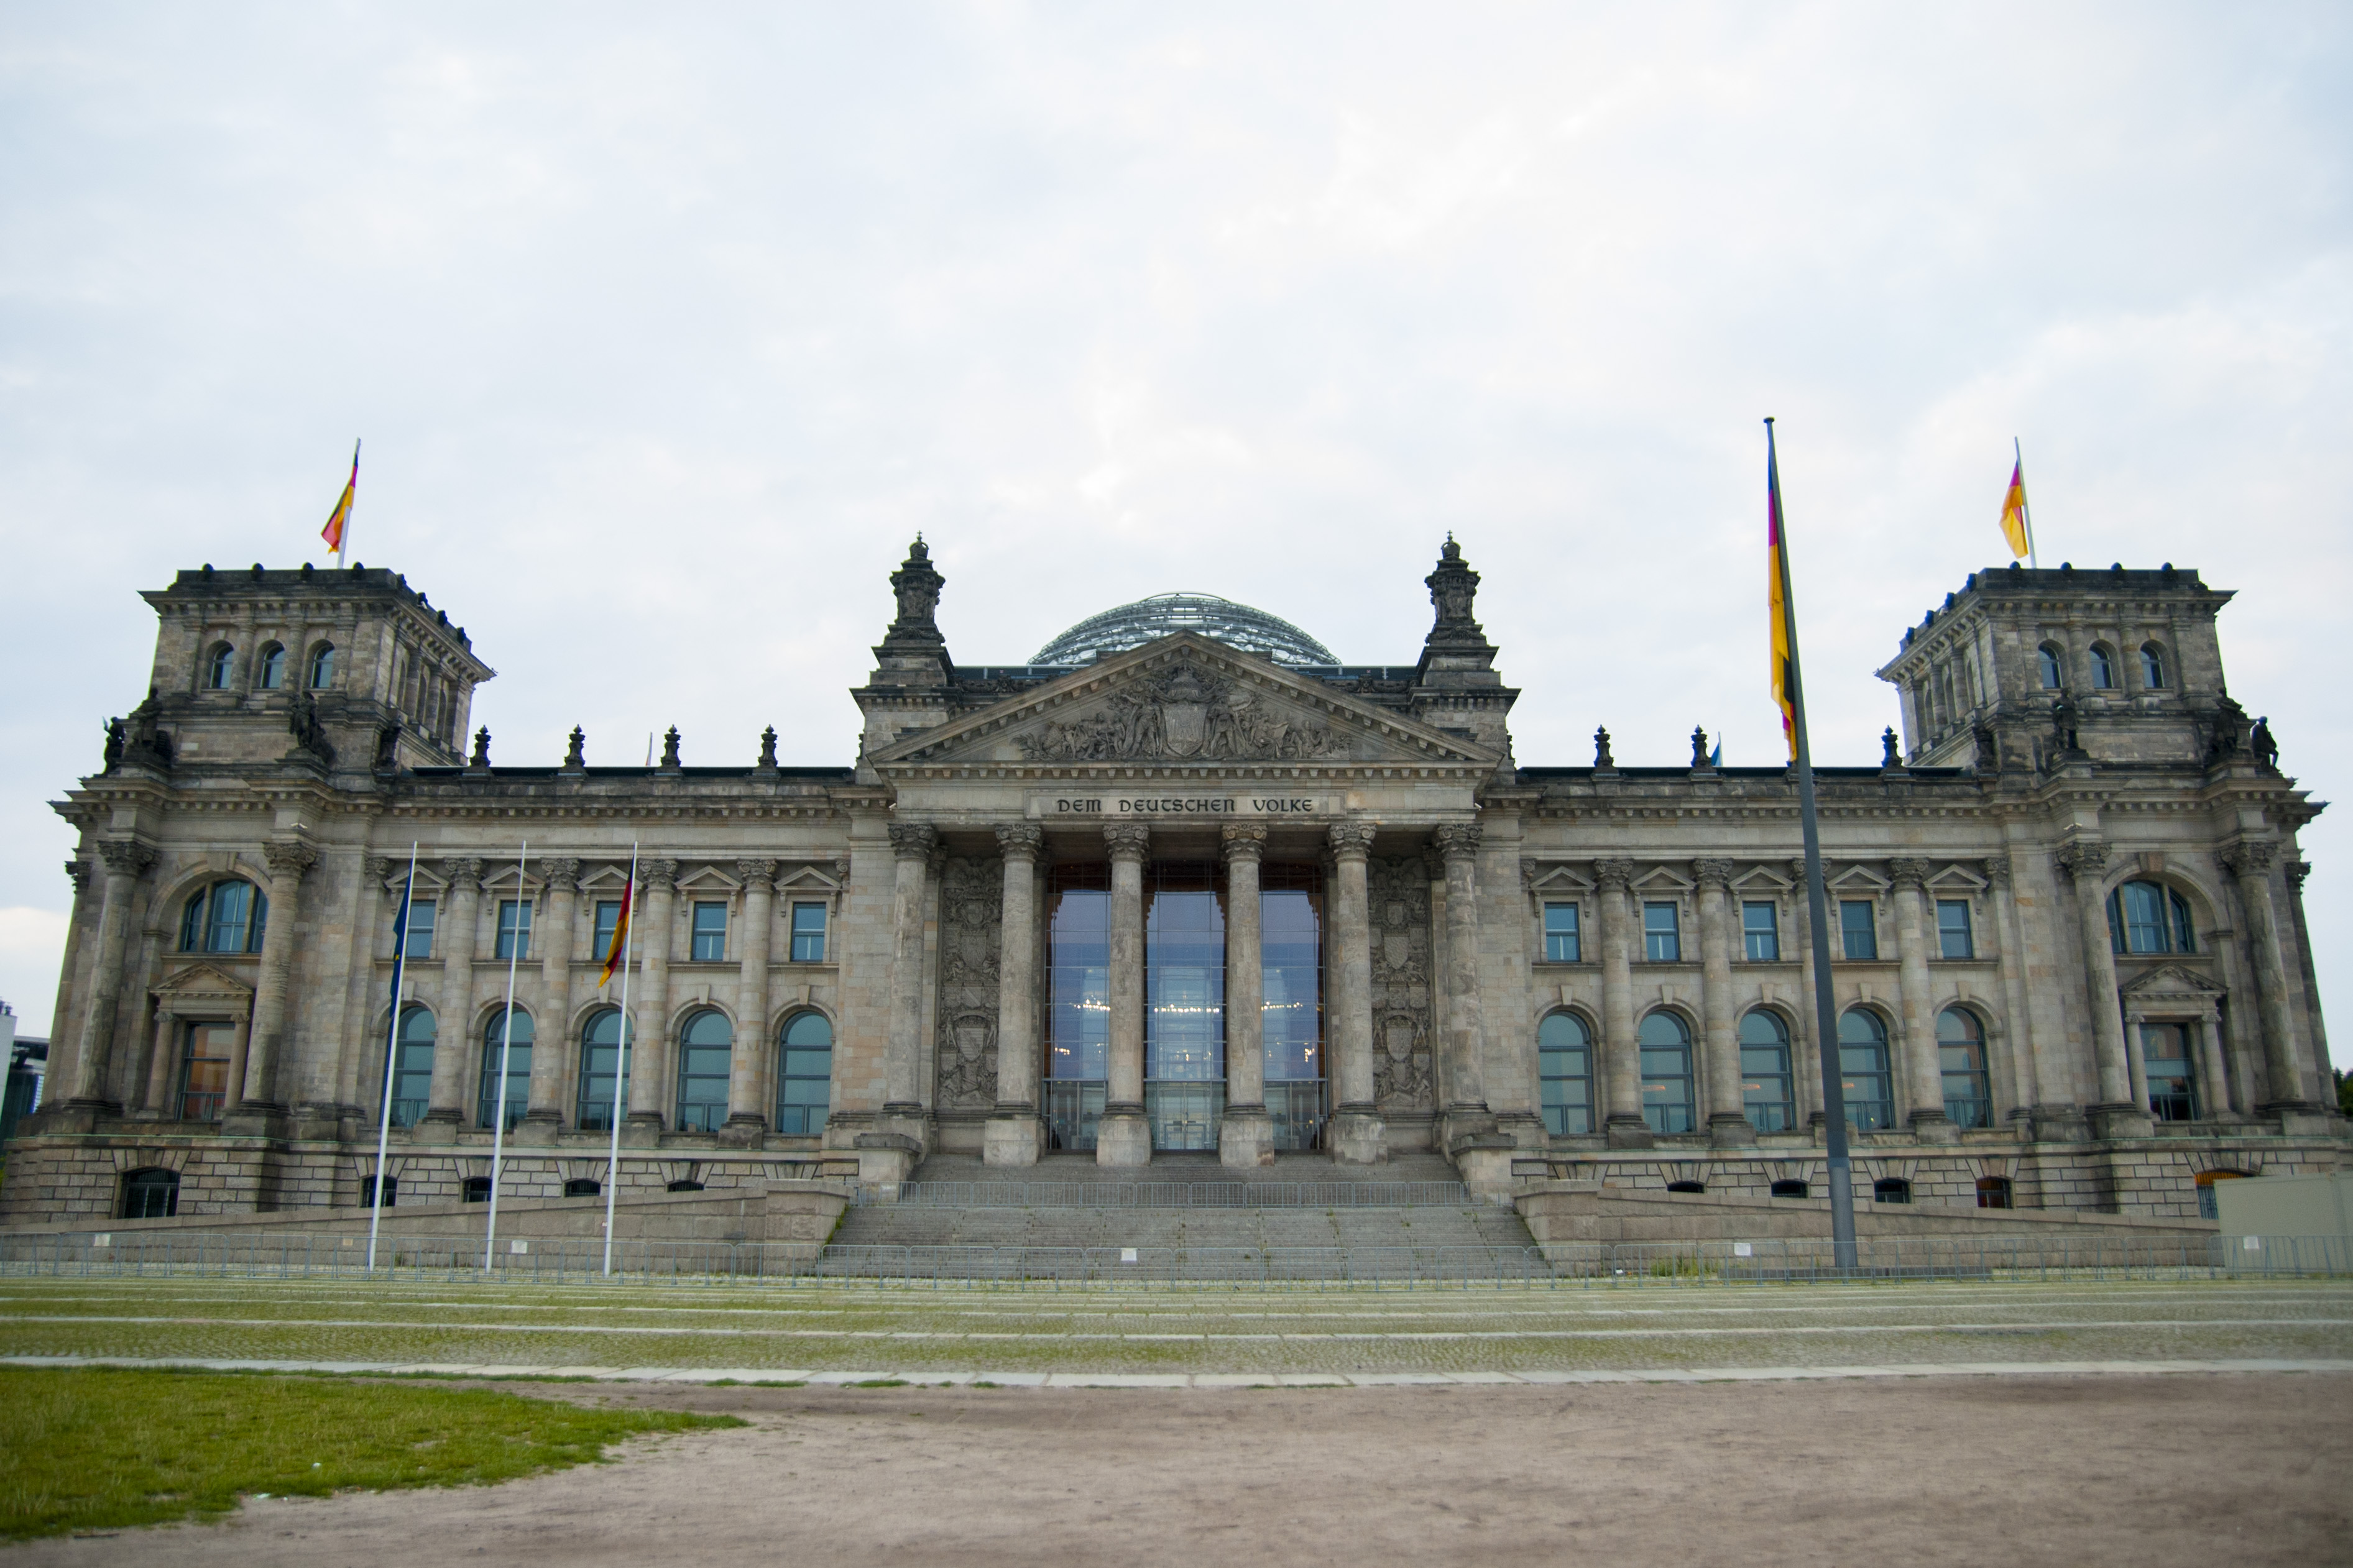
\includegraphics[width=.3\linewidth]{./figs/berlin_stuff}
   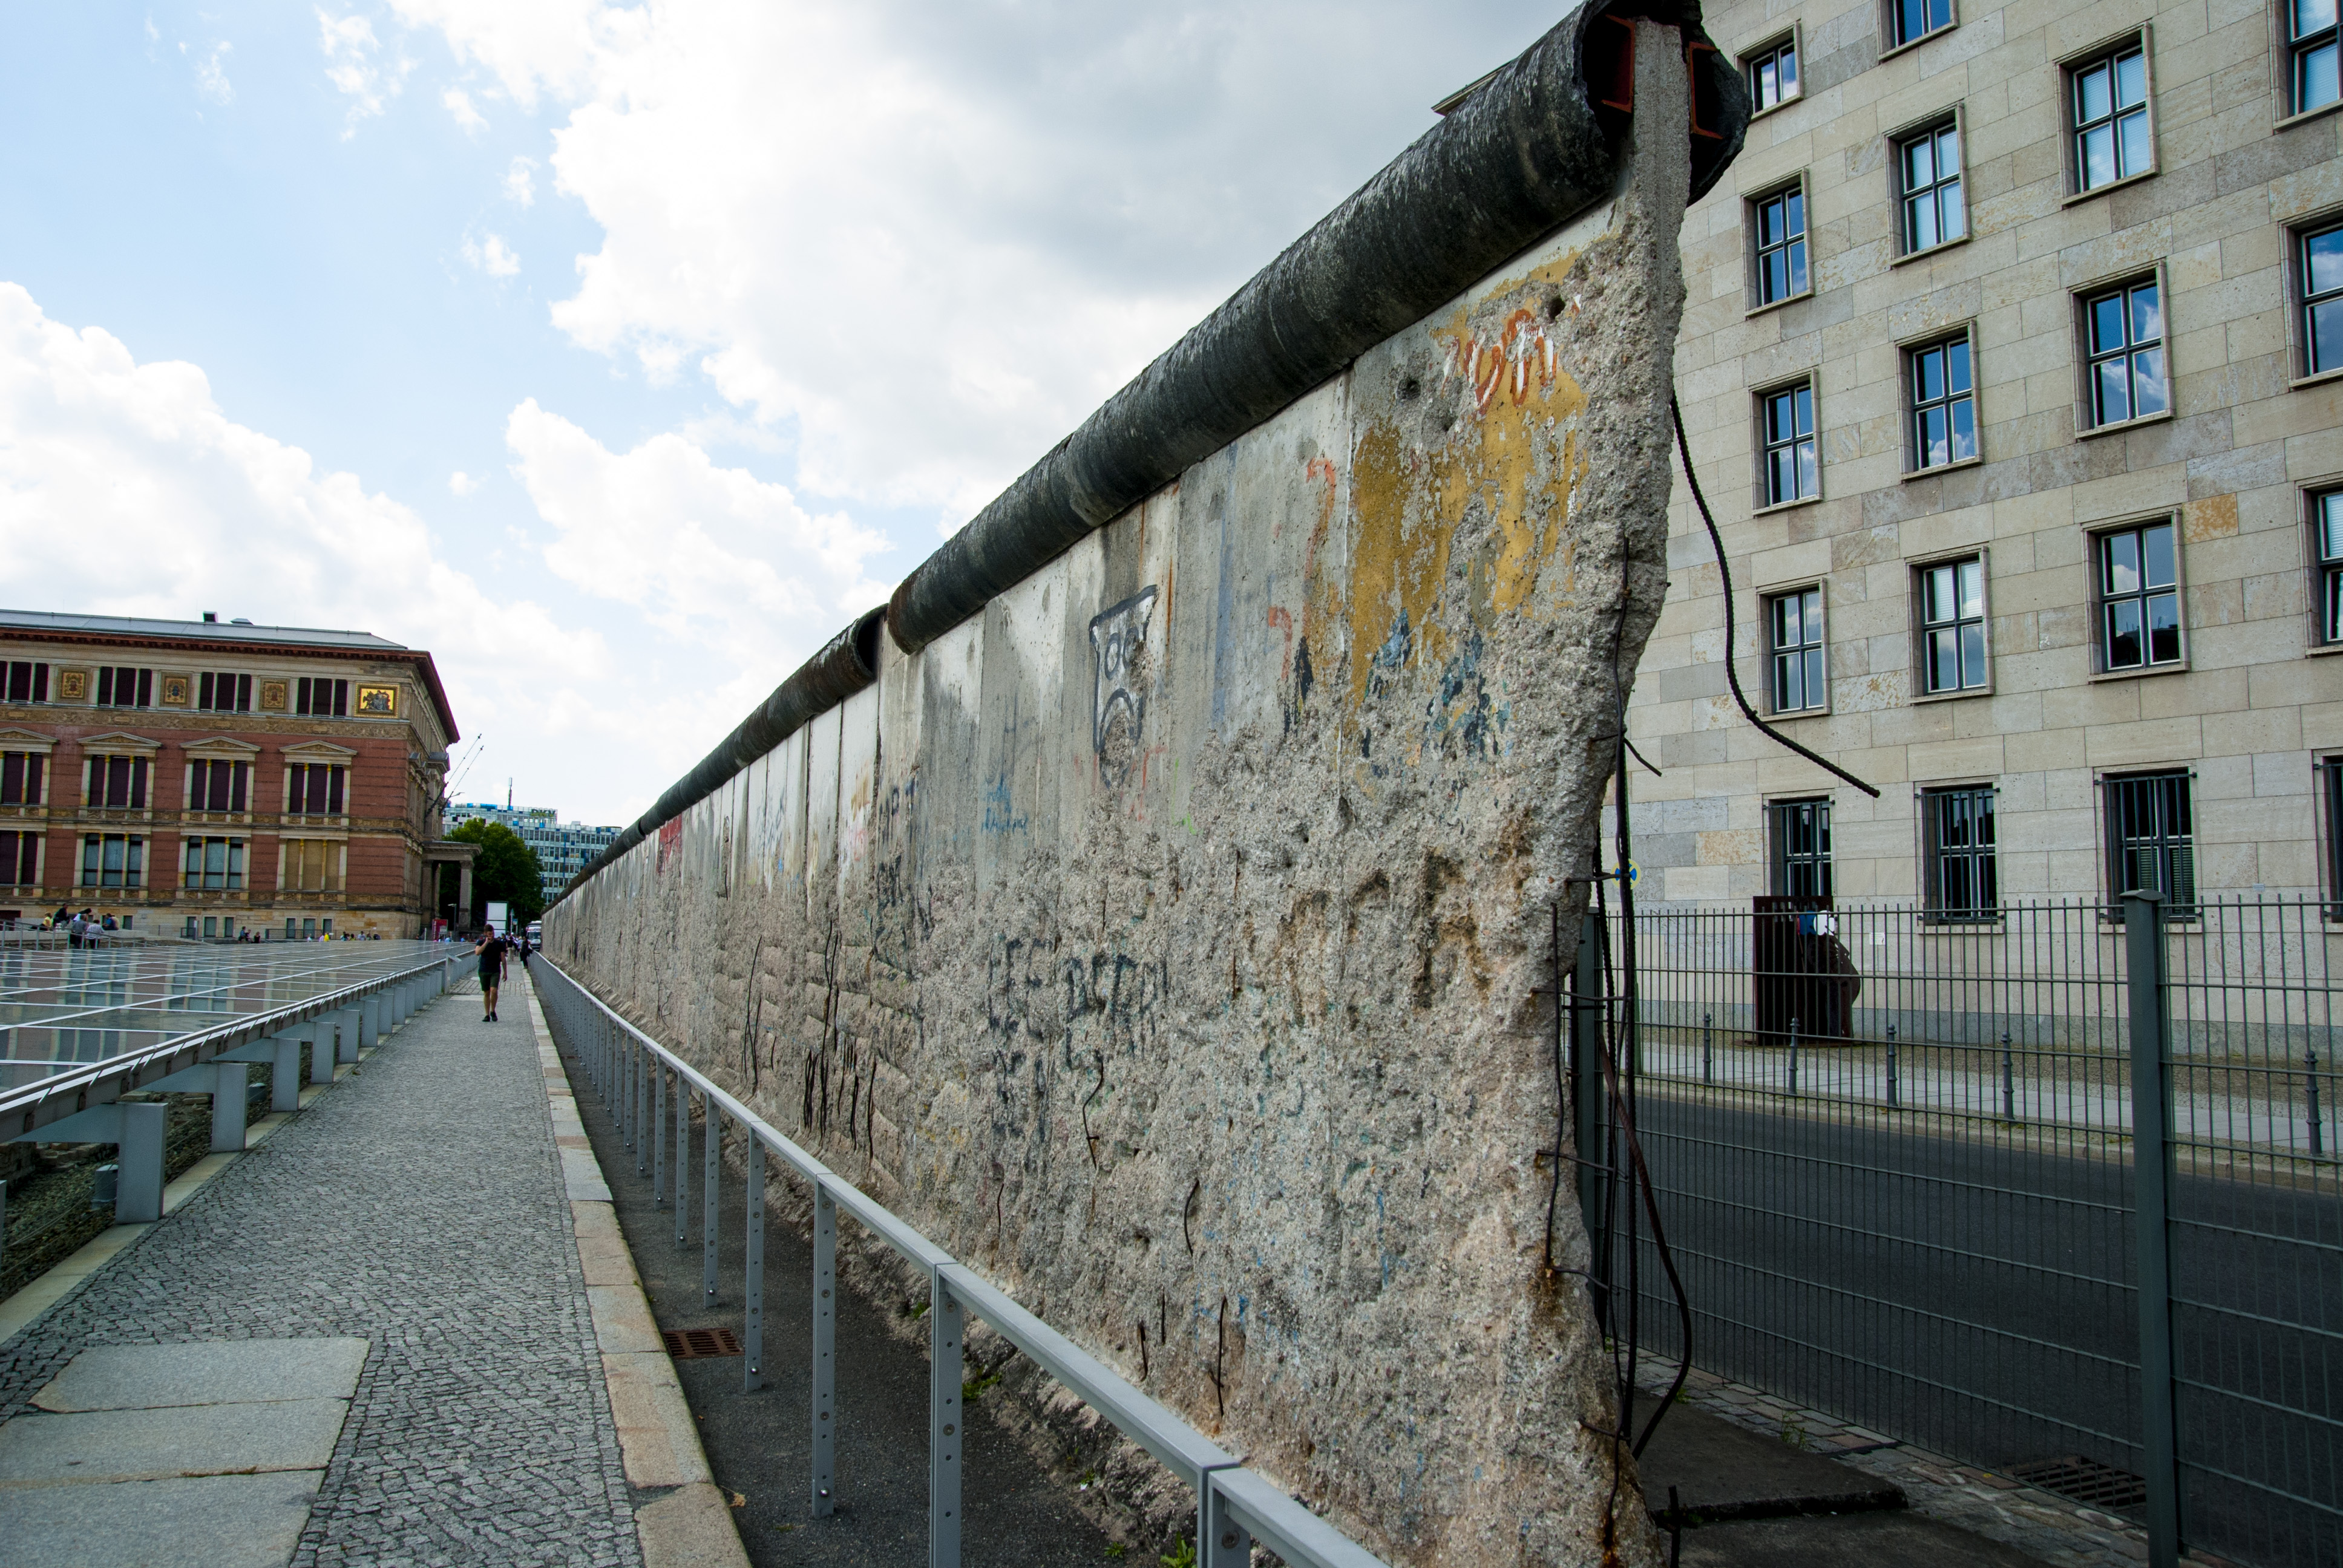
\includegraphics[width=.3\linewidth]{./figs/berlin_stuff2}
}
\end{frame}

\begin{frame}
\frametitle{What is ISU's history in the DMC}
\framesubtitle{First Place 2014}
\begin{itemize}
\item[] We had an incredible team in 2014
\item[] \centerline{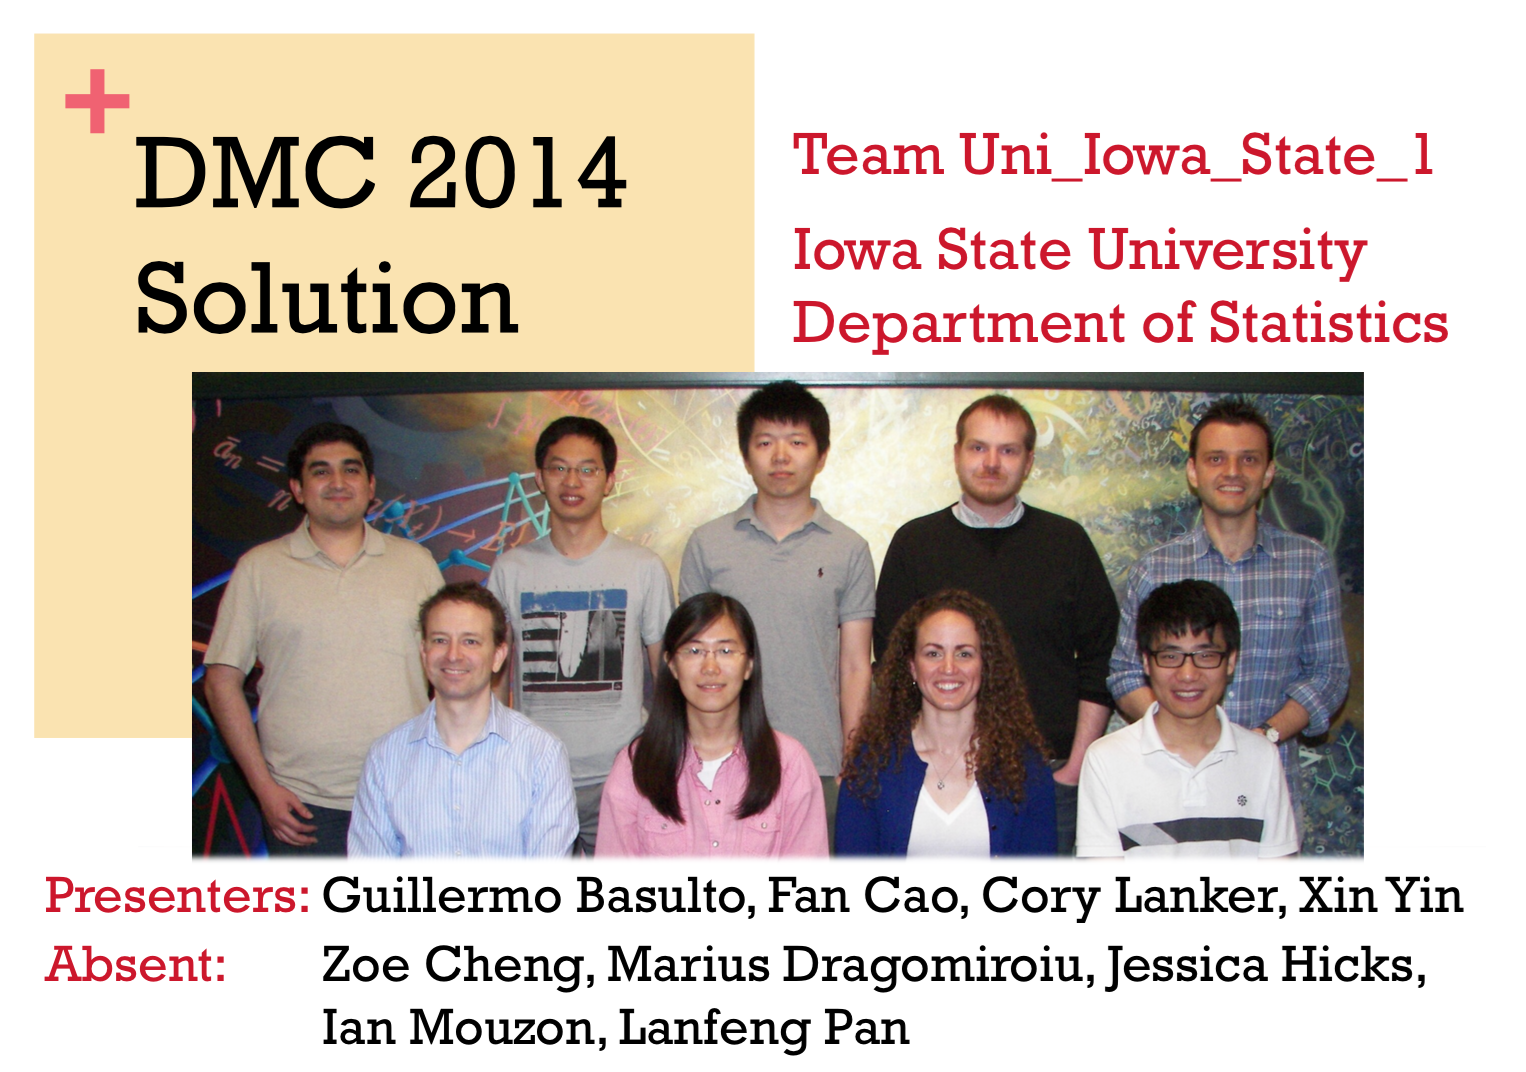
\includegraphics[width=.7\linewidth]{./figs/team2014}}
\end{itemize}
\end{frame}

\begin{frame}
\frametitle{What is ISU's history in the DMC}
\framesubtitle{First Place Goes to Germany}
\begin{itemize}
\item[] Our team in Germany
\item[] \centerline{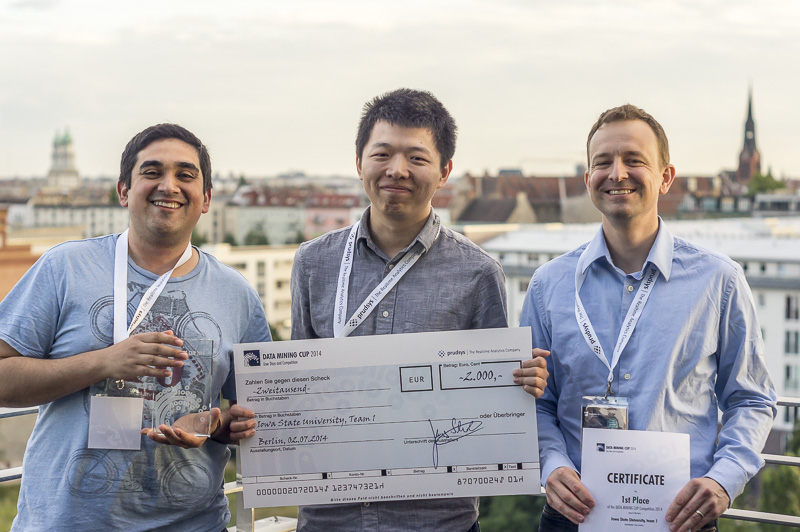
\includegraphics[width=.7\linewidth]{./figs/winners_abroad}}
\end{itemize}
\end{frame}




\begin{frame}
\frametitle{Predicting Online Orders}
\framesubtitle{The Data Mining Cup, Sponsored by prudsys}
A Data Mining Competition with two tasks:
\begin{enumerate}
   \item Use 50,000 customers session records to predict the ordering status
      of new records,
         
   \item Be able to determine in real-time whether or not a session will end
      with the customer placing an order.
\end{enumerate}
\end{frame}

\begin{frame}
   \frametitle{Overview of Dataset}
   \framesubtitle{Description of Class Variables}
   \centerline{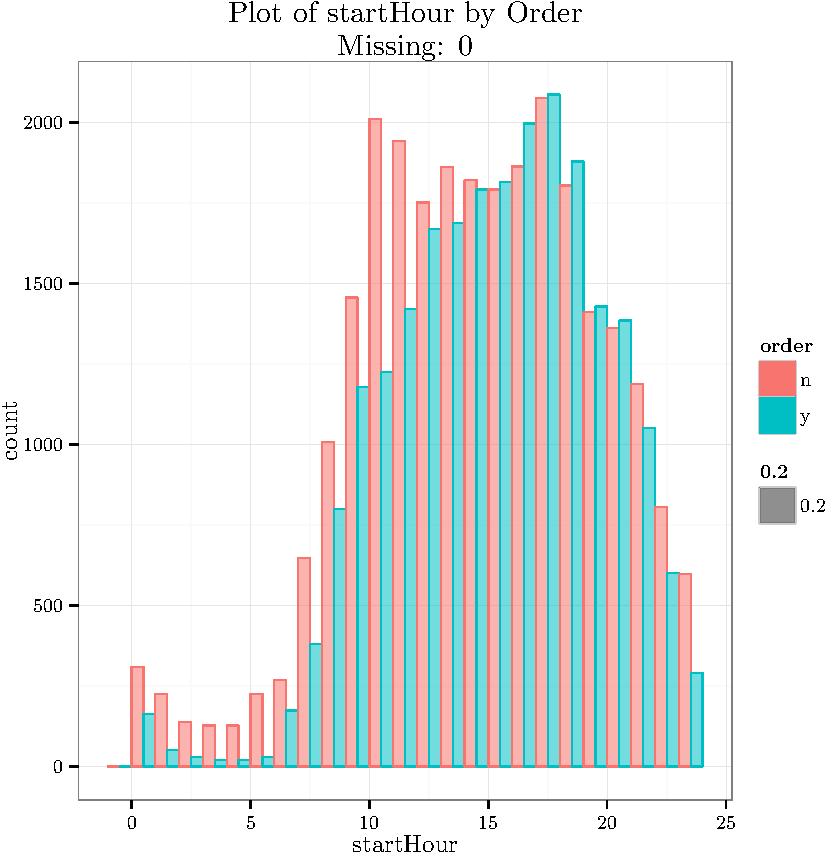
\includegraphics[width=.8\linewidth,height=.8\linewidth]{./figs/graphics-SingleDimPlot1}}
\end{frame}
\begin{frame}
   \frametitle{Overview of Dataset}
   \framesubtitle{Description of Class Variables}

   \centerline{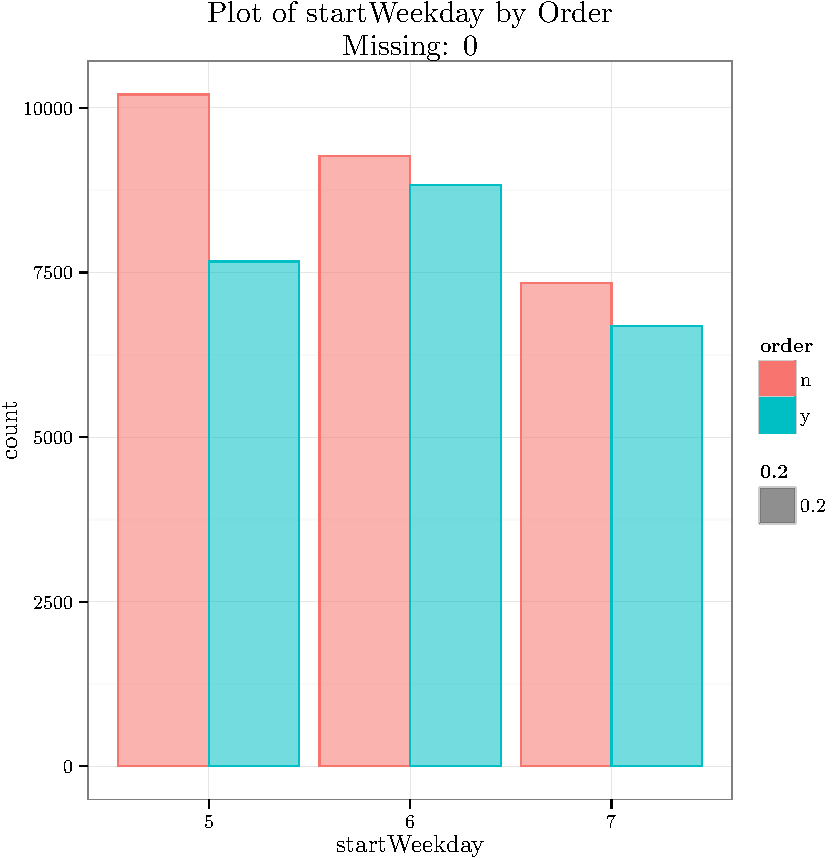
\includegraphics[width=.8\linewidth,height=.8\linewidth]{./figs/graphics-SingleDimPlot2}}
\end{frame}
\begin{frame}
   \frametitle{Overview of Dataset}
   \framesubtitle{Description of Class Variables}

   \centerline{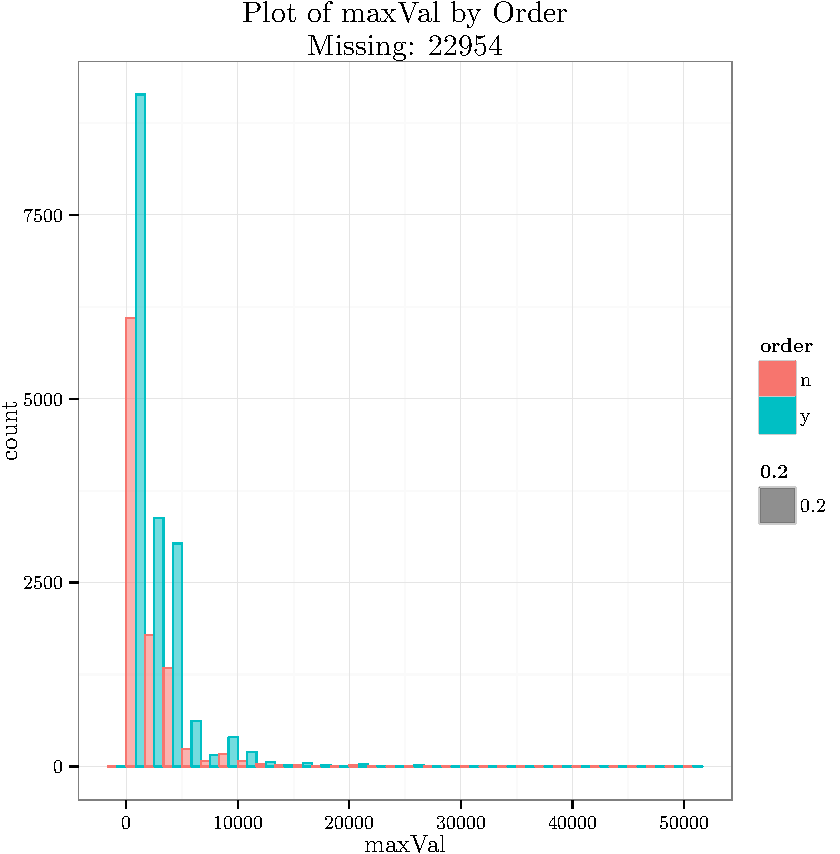
\includegraphics[width=.8\linewidth,height=.8\linewidth]{./figs/graphics-SingleDimPlot3}}
\end{frame}
\begin{frame}
   \frametitle{Overview of Dataset}
   \framesubtitle{Description of Class Variables}

   \centerline{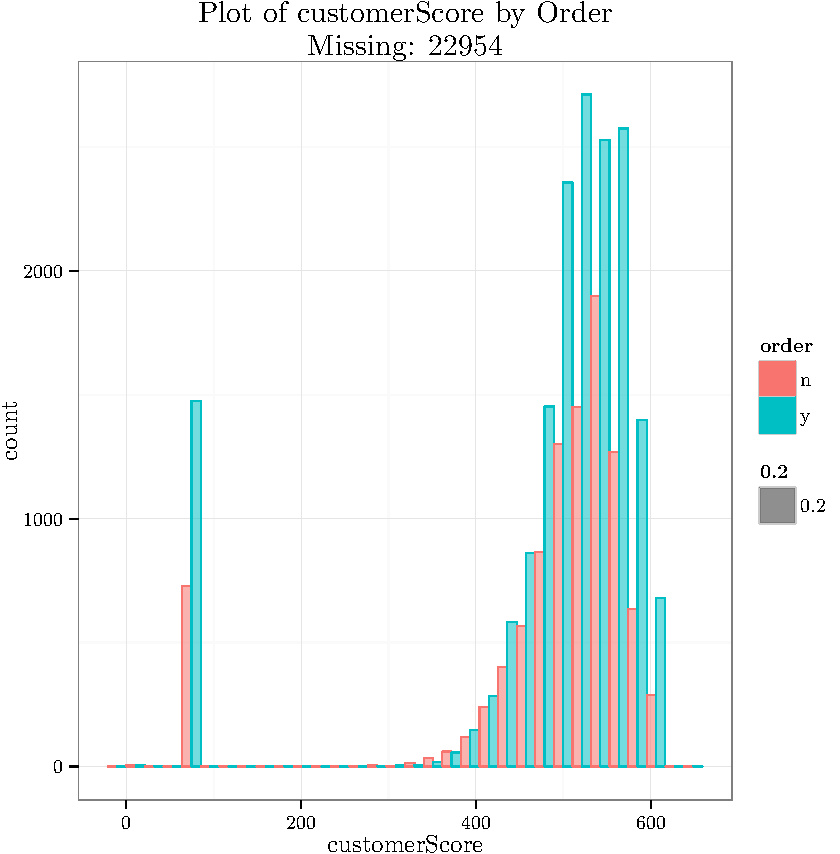
\includegraphics[width=.8\linewidth,height=.8\linewidth]{./figs/graphics-SingleDimPlot4}}
\end{frame}
\begin{frame}
   \frametitle{Overview of Dataset}
   \framesubtitle{Description of Class Variables}

   \centerline{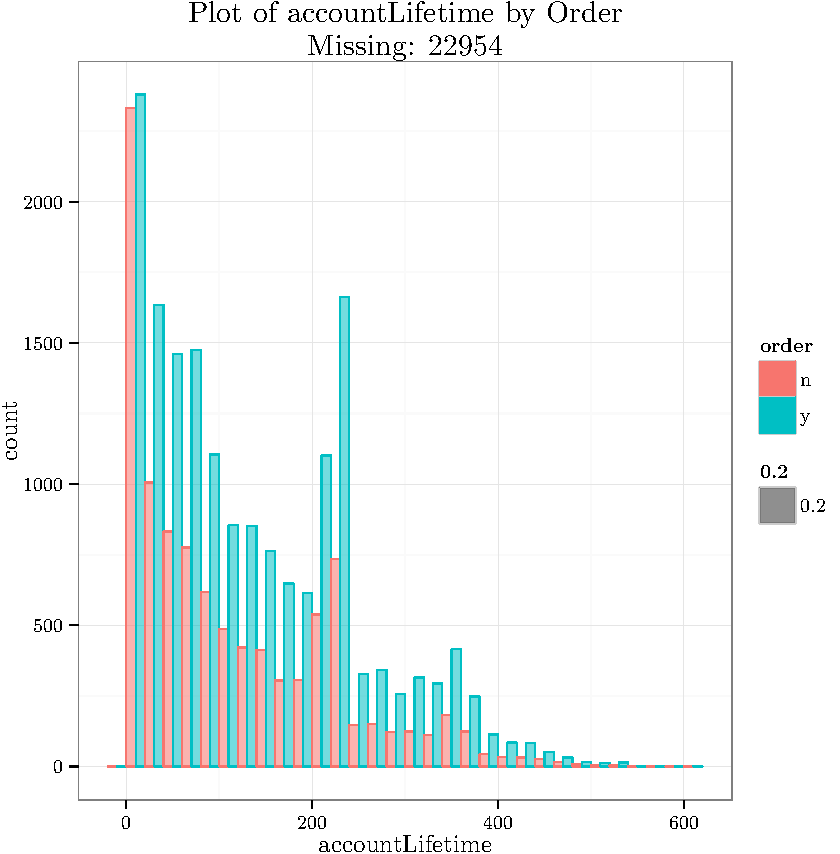
\includegraphics[width=.8\linewidth,height=.8\linewidth]{./figs/graphics-SingleDimPlot5}}
\end{frame}
\begin{frame}
   \frametitle{Overview of Dataset}
   \framesubtitle{Description of Class Variables}

   \centerline{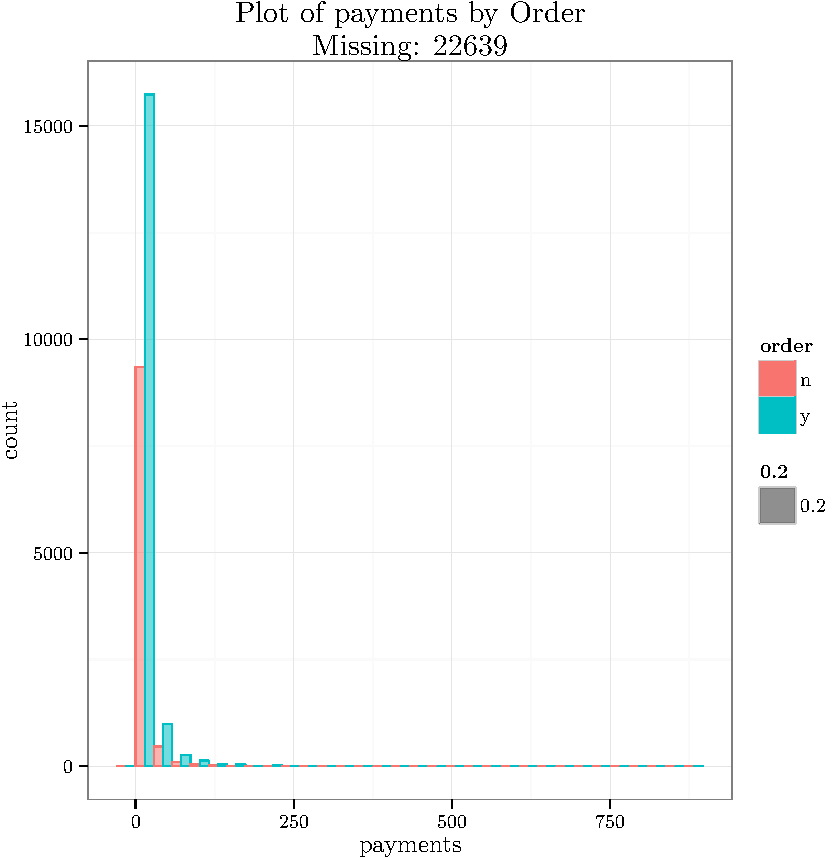
\includegraphics[width=.8\linewidth,height=.8\linewidth]{./figs/graphics-SingleDimPlot6}}
\end{frame}
\begin{frame}
   \frametitle{Overview of Dataset}
   \framesubtitle{Description of Class Variables}

   \centerline{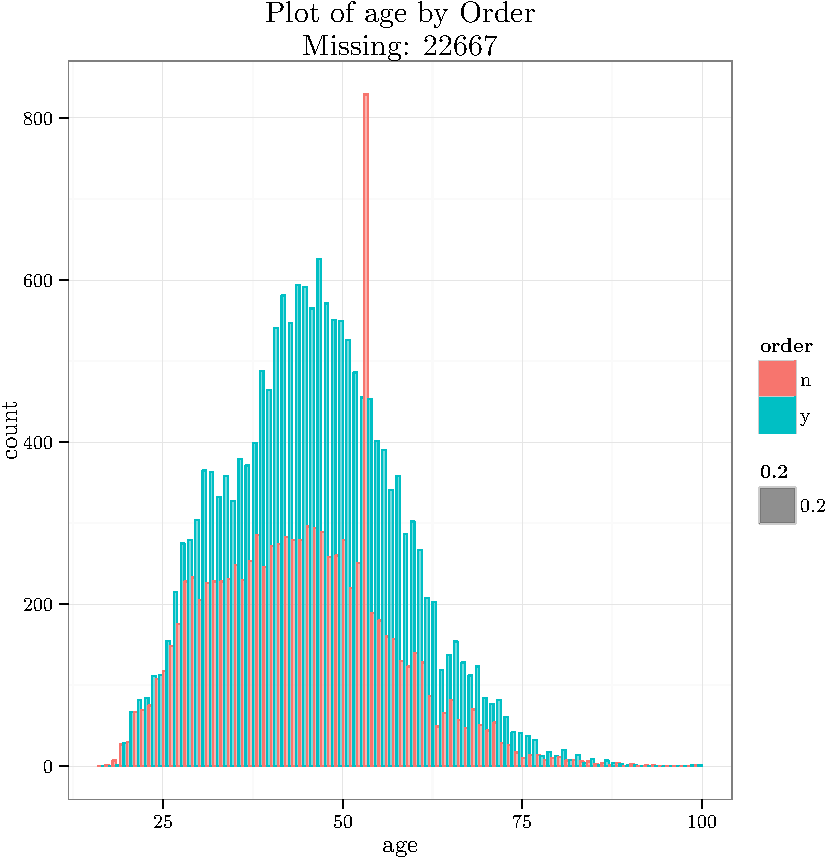
\includegraphics[width=.8\linewidth,height=.8\linewidth]{./figs/graphics-SingleDimPlot7}}
\end{frame}
\begin{frame}
   \frametitle{Overview of Dataset}
   \framesubtitle{Description of Class Variables}

   \centerline{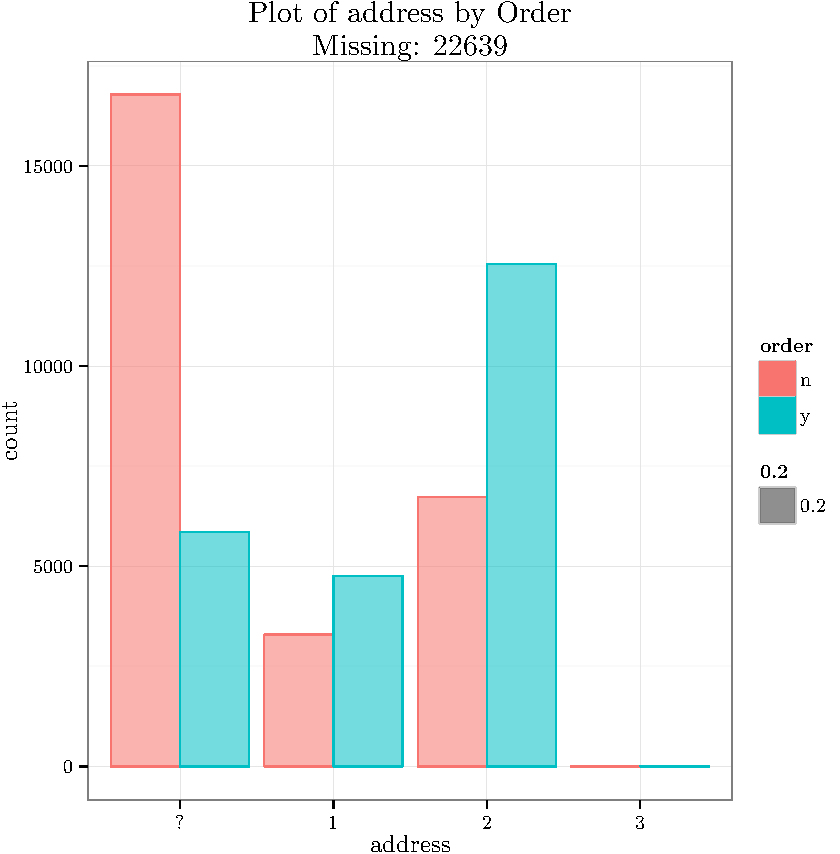
\includegraphics[width=.8\linewidth,height=.8\linewidth]{./figs/graphics-SingleDimPlot8}}
\end{frame}
\begin{frame}
   \frametitle{Overview of Dataset}
   \framesubtitle{Description of Class Variables}

   \centerline{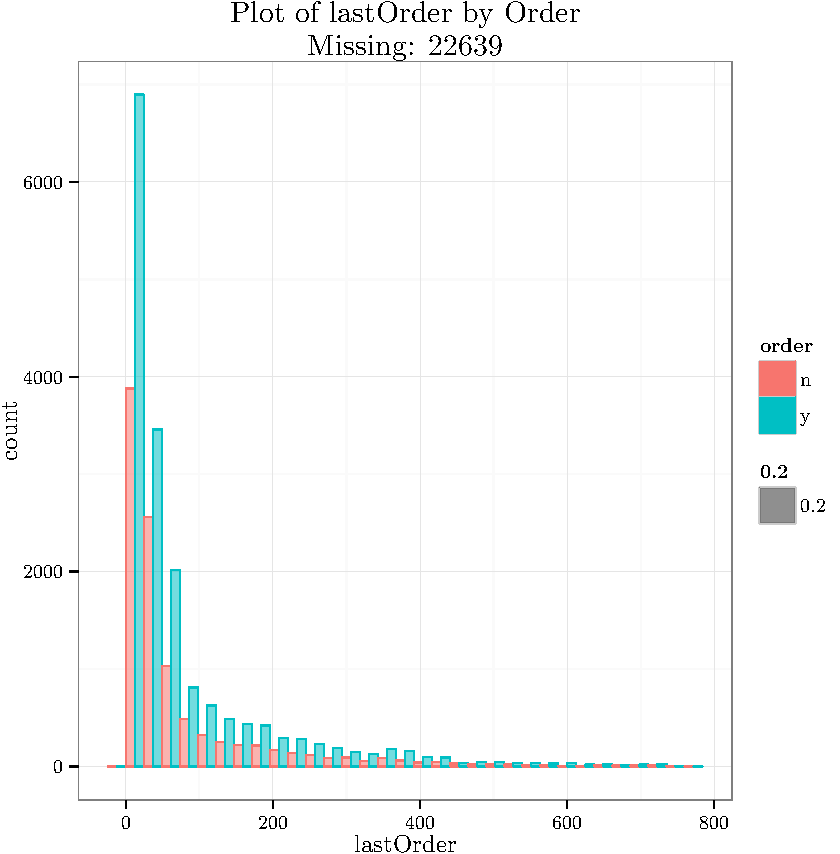
\includegraphics[width=.8\linewidth,height=.8\linewidth]{./figs/graphics-SingleDimPlot9}}
\end{frame}
\begin{frame}
   \frametitle{Overview of Dataset}
   \framesubtitle{Description of Class Variables}

   \centerline{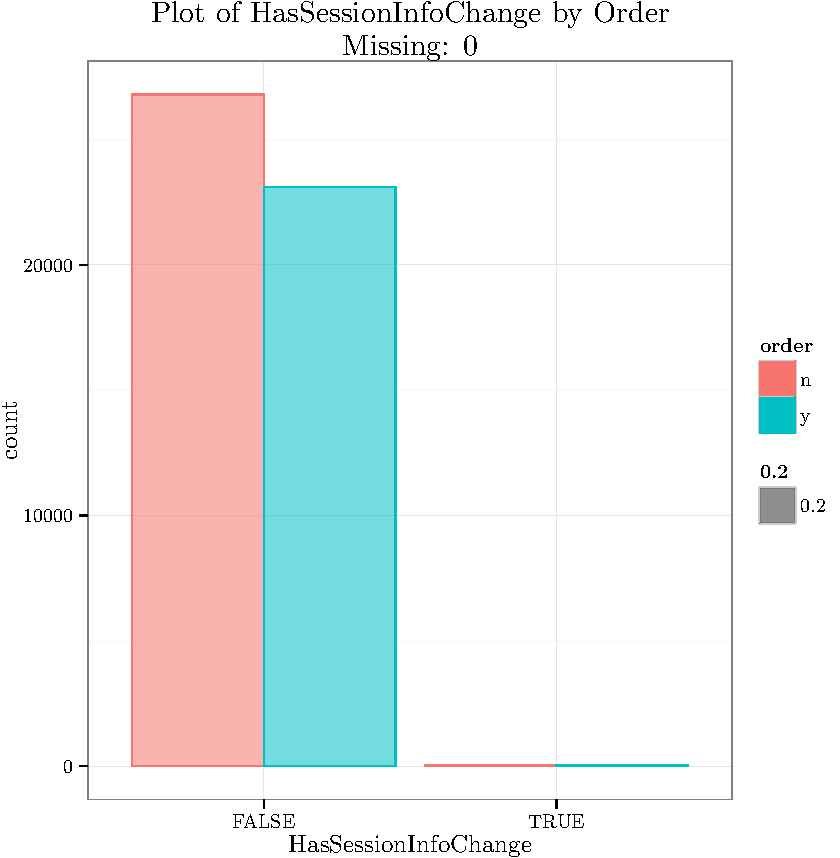
\includegraphics[width=.8\linewidth,height=.8\linewidth]{./figs/graphics-SingleDimPlot10}}

\end{frame}

\begin{frame}
   \frametitle{Overview of the Dataset}
   \framesubtitle{Key Feature: bStep}

      \centerline{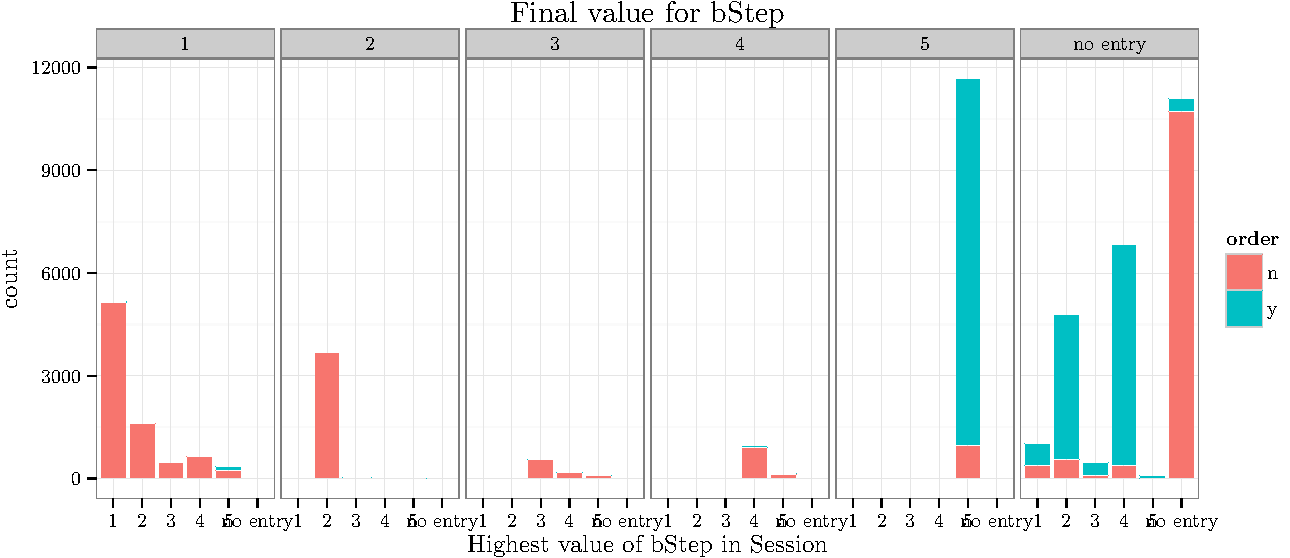
\includegraphics[width=.9\linewidth,height=.4\linewidth]{./figs/graphics-bStepPlot.pdf}}

\begin{itemize}
      \item This has split the sessions into two groups: A haystack with a few needles
         and a needle stack with a little hay.

      \item We can sort out the details using the rest of the data.
\end{itemize}
\end{frame}
\end{document}
